\documentclass[11pt,a4paper]{article}
\usepackage[T1]{fontenc}
\usepackage[utf8]{inputenc}
\usepackage{lmodern}
\usepackage[margin=1in]{geometry}
\usepackage{amsmath,amssymb,amsthm,mathtools}
\usepackage{microtype}
\usepackage{xcolor}
\usepackage{tikz}
\usetikzlibrary{arrows.meta,calc}
\usepackage[colorlinks=true,linkcolor=blue!50!black,citecolor=blue!50!black,urlcolor=blue!50!black]{hyperref}
\hypersetup{pdftitle={The crossing number of complete graphs},pdfauthor={OpenAI}}
\pdfinfoomitdate=1
\pdftrailerid{}
\pdfsuppressptexinfo=15
\newtheorem{theorem}{Theorem}[section]
\newtheorem{lemma}[theorem]{Lemma}
\newtheorem{proposition}[theorem]{Proposition}
\newtheorem{corollary}[theorem]{Corollary}
\theoremstyle{remark}
\newtheorem{remark}[theorem]{Remark}
\numberwithin{equation}{section}
\newcommand{\R}{\mathbb R}
\newcommand{\crn}{\operatorname{cr}}
\newcommand{\PP}{\mathcal P}
\newcommand{\SSS}{\mathcal S}
\newcommand{\TT}{\mathcal T}
\newcommand{\ee}{\mathbf e}
\setlength{\emergencystretch}{1.5em}

\begin{document}
\title{The crossing number of complete graphs}
\author{OpenAI}
\date{September 23, 2026}
\maketitle
\begin{abstract}
We prove the Harary--Hill conjecture: for every positive integer $n$,
the ordinary crossing number of the complete graph $K_n$ is
\[
 \frac14\left\lfloor\frac n2\right\rfloor
 \left\lfloor\frac{n-1}{2}\right\rfloor
 \left\lfloor\frac{n-2}{2}\right\rfloor
 \left\lfloor\frac{n-3}{2}\right\rfloor.
\]
\end{abstract}

\section{Introduction}

An ordinary plane drawing places the vertices of a finite simple graph
at distinct points and represents its edges by simple continuous arcs
whose interiors avoid the vertices. Edge interiors meet at finitely
many proper double crossings, with no tangencies, overlaps, or triple
crossings. Write \(c(D)\) for the number of crossing points of a drawing
\(D\), counting every crossing when two edges meet repeatedly. The
ordinary crossing number is
\[
\crn(G)=\min_D c(D).
\]
There is no restriction on vertex positions or edge routes.
The complete graph $K_n$ has one edge for each pair of its $n$ vertices.

Other crossing parameters count each intersecting edge pair once, or
count only pairs that cross an odd number of times. These objectives
differ from counting every crossing point, and restrictions on
adjacent-edge crossings affect them differently~\cite{PachToth2000,FulekEtAl2012}.
We use the ordinary point-count convention throughout.

An explicit drawing gives an upper bound on the crossing number; the
Harary--Hill problem asks whether any drawing can improve on a particular
classical construction. Harary and Hill~\cite[Section~3]{HararyHill1963}
described Hill's construction and stated the conjectured complete-graph
formula. They credited Guy's 1960 note~\cite{Guy1960} with the first
published upper bound, while noting several independent discoveries.
The distinction between curved-edge and straight-line drawings was
already explicit in their formulation.

The lower bound has developed through exact small cases, asymptotic
estimates, and the analysis of restricted drawing classes. Pan and
Richter's computer-assisted proof gave $\crn(K_{11})=100$ and hence
$\crn(K_{12})=150$~\cite{PanRichter2007}. Aichholzer subsequently
reported a computer-assisted proof of $\crn(K_{13})=225$, implying
$\crn(K_{14})=315$~\cite{Aichholzer2021}.
For general orders, de Klerk, Maharry, Pasechnik, Richter, and Salazar
used semidefinite methods to obtain an asymptotic ratio of at least
$0.83$ to the conjectured value~\cite{deKlerkEtAl2006}.
Balogh, Lidick\'y, and Salazar later proved that this ratio has limit
greater than $0.98559895$~\cite[Theorem~1]{BaloghLidickySalazar2019}.
Their use of Razborov's flag algebras~\cite{Razborov2007} constrains how
small rotation systems, which record the cyclic orders of edges at
vertices, can occur together in a large drawing.

A two-page drawing places all vertices on a line and each edge in one
of the two half-planes it bounds. Two-page constructions also attain
Hill's upper bound; their exact optimum was proved by {\'A}brego,
Aichholzer, Fern\'andez-Merchant, Ramos, and Salazar using a topological
extension of geometric edge counts~\cite{AbregoEtAl2013}.
Their subsequent shellability criterion fixes a region and an ordered
vertex set. After deleting the selected vertices outside any consecutive
subsequence of at least two vertices, its two end vertices must lie on
the boundary of the region containing the fixed one. A shelling of at
least $n/2$ vertices suffices for the conjectured lower bound.
It unifies two-page drawings with cylindrical drawings, whose vertices
lie on two concentric circles that no edge crosses, and $x$-bounded
drawings, whose edges stay between the vertical lines through their
endpoints~\cite{AbregoEtAl2014Shellable}.
Streltsova and Wagner proved the bound for vertices in general position
on the sphere joined by shortest geodesic arcs~\cite[Theorem~4]{StreltsovaWagner2025}.
These results establish the lower bound under constraints on the drawing.
Hebbar and Mangam also claimed both the complete-graph and
complete-bipartite formulas, using crossing counts for a succession
of constructed drawings~\cite[Theorems~1--3]{HebbarMangam2018}.
Counting crossings in prescribed drawings gives upper bounds;
establishing the minimum over all drawings also requires a lower-bound
argument.
We prove the following formula for unrestricted ordinary drawings.

\begin{theorem}\label{thm:main}
For every integer \(n\ge3\),
\[
\crn(K_n)=Z(n):=
\frac14\left\lfloor\frac n2\right\rfloor
\left\lfloor\frac{n-1}2\right\rfloor
\left\lfloor\frac{n-2}2\right\rfloor
\left\lfloor\frac{n-3}2\right\rfloor.
\]
\end{theorem}

Thus Theorem~\ref{thm:main} resolves the Harary--Hill conjecture
positively. The cases \(n=1,2\) have crossing-free drawings and the
same floor product is zero. In parity-specific form the value is
\begin{equation}\label{eq:parity}
Z(2s+1)=\binom{s}{2}^{\!2},
\qquad
Z(2s)=\frac{s(s-1)^2(s-2)}4.
\end{equation}

Our lower bound uses algebraic information about a drawing rather than
a restriction on its edge routes. Tutte developed an algebraic theory
of crossing numbers~\cite{Tutte1970}. Woodall's cyclic-order graphs use
the orders of incident edges, and distances between those orders, to
bound crossings in complete-bipartite drawings~\cite[Sections~2--3]{Woodall1993}.
Here signed intersections retain the orientation of each crossing.
Together with the local orders, they enter a corrected bilinear pairing
that vanishes on pairs of cycles. Polynomial interpolation then turns
this identity into a crossing lower bound.

For the odd case $n=2s+1$, choose a distinct real label for each vertex.
We use polynomials in four variables, representing the endpoints of two
edges. Each polynomial is symmetric in the endpoints of either edge and
has degree at most $s-2$ in each variable. This space has dimension
$Z(2s+1)$. Evaluate its members at every ordered pair of independent
edges with a nonzero signed crossing count. The central task is to show
that these evaluations determine the polynomial.

The accompanying bipartite paper develops an odd-node order
detector~\cite[Section~4]{BipartiteCompanion}.
Here an even-node detector, built from the classical Lagrange
weights~\cite[Sections~2--3]{BerrutTrefethen2004}, recovers local information
at each vertex from the cycle identity. It forces a polynomial in the
kernel of the evaluation map to vanish whenever endpoints of different
edges coincide. The resulting difference factors can be divided out
while preserving both the kernel and the endpoint symmetries. Repetition
would lower the degree indefinitely, so the kernel is zero.

A second application of the cycle identity, now multiplied by the
product of all six endpoint differences, shows that the evaluation
image is totally isotropic: every two image vectors pair to zero in a
nondegenerate symmetric diagonal form. The standard orthogonal-complement
dimension formula bounds this image by half the number of its coordinates.
Each supported unordered edge pair requires a crossing, yielding the
odd lower bound. Vertex deletion gives the even case. The needed geometry
and algebra are proved locally; the detector works for every order of
arbitrary distinct real nodes.

The lower bound does not depend on the bipartite crossing-number
formula. Section~\ref{sec:cycles} establishes
the geometric identity; Sections~\ref{sec:interpolation}
and~\ref{sec:lower} prove the lower bound; Section~\ref{sec:upper}
gives the matching construction. Appendix~\ref{sec:normalization}
supplies the reduction from continuous arcs.

\section{Signed intersections of cycles}\label{sec:cycles}

Our first goal is an identity relating interior crossings to the circular
orders of edges at vertices. We will apply it to polynomially weighted
cycles in Section~\ref{sec:lower}.

By Lemma~\ref{lem:normalization}, a minimum drawing can be chosen
polygonal, straight near every vertex and crossing, and without
crossings between adjacent edges. We call such a drawing \emph{normalized}.
Independent edges may still cross more than once.

Fix one orientation of each edge of a finite simple graph drawn in this way.
Its real edge space has those oriented edges as a basis. Reversing an
orientation negates the edge vector. For \(K_n\) we write \([ip]\) for
the edge from \(i\) to \(p\), so \([pi]=-[ip]\) and \([ii]=0\).
The boundary map is
\(\partial[ip]=\ee_p-\ee_i\), with the vertex symbols as a basis.
A \emph{cycle} is a chain in \(\ker\partial\).

Let \(I(e,f)\) be the sum of the signs of the interior crossings of
two distinct oriented basis edges. The sign is positive when their
ordered tangent directions give the positive orientation of the plane.
Set \(I(e,e)=0\). At each vertex \(w\), choose a gap in the circular
order of the outward spokes and list the incident edges
counterclockwise from it. Put
\[
T_w(e,f)=
\begin{cases}
1,&e\text{ precedes }f,\\
-1,&f\text{ precedes }e,\\
0,&e=f,
\end{cases}
\qquad
\sigma_{we}=
\begin{cases}
1,&e\text{ points out of }w,\\
-1,&e\text{ points into }w.
\end{cases}
\]
Define a bilinear form by its values on basis edges:
\begin{equation}\label{eq:J}
J(e,f)=I(e,f)+\frac12
\sum_{\substack{w\text{ an endpoint}\\\text{of both }e,f}}
\sigma_{we}\sigma_{wf}T_w(e,f).
\end{equation}
It is skew-symmetric. The orientation signs in
Equation~\eqref{eq:J} make its bilinear extension consistent with
reversing either edge.

\begin{lemma}[Cycle pairing]\label{lem:cycles}
For any two cycles \(z,z'\), one has \(J(z,z')=0\).
\end{lemma}

\begin{proof}
The following argument also appears in the companion paper
\cite[Lemma~3.1]{BipartiteCompanion}; it applies to every finite simple graph.
The kernel of the boundary map is spanned by signed simple graph
cycles. Indeed, choose a spanning forest, subtract the fundamental
cycle associated with each nonforest edge with its appropriate
coefficient, and obtain a cycle supported on a forest. Stripping
leaves shows that the remaining chain is zero. It therefore suffices
to treat two oriented simple graph cycles.

We will replace the first cycle by a closed polygonal walk \(\gamma\)
and the second by two closed polygonal walks \(\eta_+,\eta_-\).
The average of the signed intersection counts of \(\gamma\) with
these two walks will be \(J(z,z')\): crossings outside small vertex
disks contribute \(I\), while the averaged contributions inside them
give the correction in Equation~\eqref{eq:J}. Each total intersection
count is zero, as we prove at the end of the argument.

\emph{The local contribution.} Consider two oriented chords \(C,E\) of a round disk, with
four distinct boundary endpoints. Give a chord's start coefficient
\(-1\) and its end coefficient \(+1\), denoted by \(\epsilon_C\)
and \(\epsilon_E\). If \(T(u,v)\) compares boundary points from a
counterclockwise cut away from the endpoints, their signed intersection is
\begin{equation}\label{eq:chord}
I(C,E)=\frac12
\sum_{u\in\partial C}\sum_{v\in\partial E}
\epsilon_C(u)\epsilon_E(v)T(u,v).
\end{equation}
Moving the cut past one endpoint changes the right side by a multiple
of the other chord's total endpoint coefficient, which is zero.
Cutting just before the start of \(C\), the expression becomes minus
the sum of \(\epsilon_E\) on the open counterclockwise boundary arc
from the start to the end of \(C\). This arc is on the right of the
directed chord. The expression is zero for nonalternating endpoints,
and is \(+1\) for \(E\) crossing from right to left, or \(-1\) for
the reverse. These are exactly the intersection signs. Figure~\ref{fig:local-pairing}
shows this convention and the shared-spoke averaging used below.

\begin{figure}[tbp]
\centering
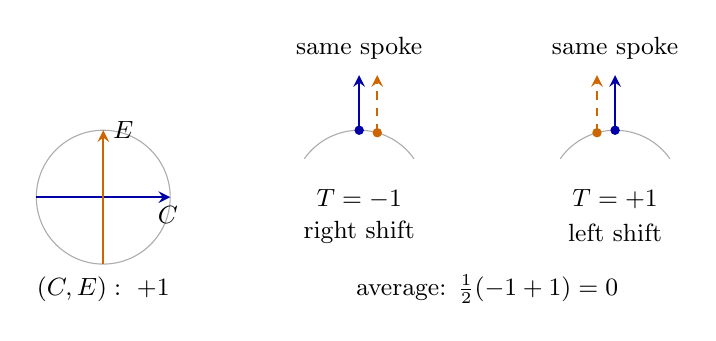
\begin{tikzpicture}[x=1cm,y=1cm,>=stealth,font=\small,
  first/.style={draw=blue!65!black,line width=.85pt},
  second/.style={draw=orange!80!black,line width=.85pt}]
  \begin{scope}
    \draw[gray!65] (0,0) circle (.85);
    \draw[first,->] (-.85,0)--(.85,0);
    \draw[second,->] (0,-.85)--(0,.85);
    \node[below right] at (.57,0) {$C$};
    \node[above right] at (0,.62) {$E$};
    \node at (0,-1.17) {$(C,E):\ +1$};
  \end{scope}
  \begin{scope}[xshift=3.25cm]
    \draw[gray!65] (145:.85) arc (145:35:.85);
    \draw[first,->] (0,.85)--(0,1.55);
    \draw[second,dashed,->] (.23,.8185)--(.23,1.55);
    \fill[blue!65!black] (0,.85) circle (1.7pt);
    \fill[orange!80!black] (.23,.8185) circle (1.7pt);
    \node at (0,-.02) {$T=-1$};
    \node at (0,-.45) {right shift};
    \node[above] at (0,1.63) {same spoke};
  \end{scope}
  \begin{scope}[xshift=6.5cm]
    \draw[gray!65] (145:.85) arc (145:35:.85);
    \draw[first,->] (0,.85)--(0,1.55);
    \draw[second,dashed,->] (-.23,.8185)--(-.23,1.55);
    \fill[blue!65!black] (0,.85) circle (1.7pt);
    \fill[orange!80!black] (-.23,.8185) circle (1.7pt);
    \node at (0,-.02) {$T=+1$};
    \node at (0,-.45) {left shift};
    \node[above] at (0,1.63) {same spoke};
  \end{scope}
  \node at (4.875,-1.17) {average: $\tfrac12(-1+1)=0$};
\end{tikzpicture}
\caption{The local signs in the cycle pairing. Left: a chord directed to
the right followed by one directed upward gives a positive crossing.
Right: alternative right and left displacements of the second track at
a shared spoke give opposite comparisons in counterclockwise boundary
order. The two displacements are alternative perturbations whose counts are averaged.}
\label{fig:local-pairing}
\end{figure}


\emph{Separating shared tracks.} Choose disjoint small round vertex disks
meeting only the straight spokes. In each vertex disk replace the first cycle's passage by the
chord from its incoming to its outgoing boundary point. Outside
these disks retain its edge tracks, obtaining a closed polygonal
walk \(\gamma\).

Construct two versions \(\eta_+,\eta_-\) of the second cycle.
Outside the vertex disks, displace each track slightly left or right,
respectively, relative to its fixed basis-edge orientation. In the
vertex disks join its displaced endpoints by chords. Here are the
local details needed when the cycles share edges. Place additional
disjoint small round disks at crossings and nonstraight bends,
meeting only their incident straight pieces. Shift each straight
stretch between disks to a parallel one. Across a crossing disk
continue along the shifted line: it avoids its own original line
and crosses the other original strand once, with the same sign.
At a bend the shifted ends lie on the same side of the original
bent track. For a left shift they lie clockwise of its incoming
outward ray and counterclockwise of its outgoing ray. Join them
by a polygonal path in that component of the bend disk; use the
other component for a right shift.

The distinct truncated stretches between disks are compact and
disjoint. Finiteness therefore permits a common sufficiently small
shift introducing no additional intersections. The vertex cuts and
comparisons between distinct spokes remain unchanged. At seams the
shifted and original endpoints are distinct; chord interiors stay
inside their disks, and the intended crossings remain strictly
inside crossing disks. These local replacements join to closed
polygonal walks \(\eta_+,\eta_-\). Every intersection between
\(\gamma\) and either walk is transverse and lies away from their
corners; unnecessary straight subdivision points can be removed.

In either version the signed intersection count outside the vertex
disks, counting by traversals, is
\[
\sum_{e,f}z_ez'_f I(e,f).
\]
This remains true for shared tracks: a shifted edge avoids its own
copy, and crossings of different edges give the two ordered
contributions when both cycles use both edges.

In a common vertex disk the first chord's endpoint coefficient on
spoke \(e\) is \(\sigma_{we}z_e\): an incoming traversal starts the
chord and an outgoing traversal ends it. The second chord has
coefficient \(\sigma_{wf}z'_f\). For distinct spokes, the comparison
sign in Equation~\eqref{eq:chord} is \(T_w(e,f)\) for both shifts.
For a shared spoke the two shifted endpoints are on opposite sides
of its original endpoint, so their comparison signs average to zero.
The average vertex contribution is therefore
\[
\frac12\sum_{e,f\text{ incident with }w}
z_ez'_f\sigma_{we}\sigma_{wf}T_w(e,f).
\]
Opposite cycle traversals change the coefficients, not this averaging.
In particular, for opposite traversals of a shared edge, the same
coefficient multiplies both opposite shared-spoke comparisons,
whose average remains zero.

\emph{Total signed intersection.} Two closed polygonal walks in the plane
that meet transversely away from their corners have total signed
intersection zero, with intersections counted by traversals.
To see this without a simplicity assumption, cone every oriented
segment \([u,v]\) of the first walk to a common point \(o\), forming
the oriented triangle \([o,u,v]\). Choose \(o\) outside the finitely
many lines that cause degeneracy, a cone segment to pass through a
corner of the second walk, or nontransverse intersections.
Each triangle boundary has total signed intersection zero: along
the closed second walk, entrances and exits have opposite signs.
In the sum of the triangle boundaries the extra cone sides cancel,
leaving the first walk. This proves the assertion.

Apply it to \((\gamma,\eta_+)\) and \((\gamma,\eta_-)\) and average.
The exterior and vertex contributions just computed sum to
\(J(z,z')\), proving the lemma.
\end{proof}

\section{An even-node order detector}\label{sec:interpolation}

The cycle identity retains the order of the spokes at each vertex.
We next show that this order, combined with interpolation weights,
detects a polynomial from its pairings with a prescribed test space.
The prescribed order need not agree with the numerical order of the nodes.

For nonnegative integers \(a,b\), let \(\PP_{a,b}\) be the real
polynomials in \(u,v\) of degrees at most \(a,b\) separately.

\begin{lemma}[Interpolation weights]\label{lem:weights}
For distinct real nodes \(u_1,\ldots,u_N\), put
\(G(t)=\prod_{p=1}^{N}(t-u_p)\). Then
\[
\sum_{p=1}^{N}\frac{A(u_p)}{G'(u_p)}=0
\qquad\text{if }\deg A\le N-2.
\]
\end{lemma}

\begin{proof}
The Lagrange formula
\[
A(t)=\sum_p A(u_p)\frac{G(t)}{(t-u_p)G'(u_p)}
\]
holds for \(\deg A\le N-1\): both sides have degree at most \(N-1\)
and agree at all \(N\) nodes. Comparing coefficients of \(t^{N-1}\)
gives the assertion.
\end{proof}

The next lemma is an even-node counterpart of the two-triangle
interpolation used in \cite[Section~4]{BipartiteCompanion}. Its two degree
rectangles exchange roles in the induction.

\begin{lemma}[Two-triangle interpolation]\label{lem:triangles}
Let \(s\ge2\) and let \(u_1,\ldots,u_{2s}\) be distinct real numbers.
Set
\[
L_s=\{(p,q):1\le q<p\le s\}
\;\cup\;\{(p,q):s<p<q\le2s\}.
\]
Evaluation at \((u_p,u_q)\), \((p,q)\in L_s\), is an isomorphism
from each of \(\PP_{s-1,s-2}\) and \(\PP_{s-2,s-1}\) onto
\(\R^{L_s}\).
\end{lemma}

\begin{proof}
Both spaces and the target have dimension \(s(s-1)\), so it suffices
to prove injectivity, simultaneously for the two spaces.
For \(s=2\), the two points have distinct first coordinates and
distinct second coordinates. They determine an affine polynomial
in either one variable.

For larger \(s\), let \(P\in\PP_{s-1,s-2}\) vanish on the pattern.
Each of the rows \(p=s,s+1\) contains \(s-1\) points. Thus the
polynomials \(P(u_s,v)\) and \(P(u_{s+1},v)\), of degree at most
\(s-2\), vanish identically. It follows that
\[
P(u,v)=(u-u_s)(u-u_{s+1})R(u,v),
\qquad R\in\PP_{s-3,s-2}.
\]
Remove those two indices from the node list. The remaining two
triangles are the pattern \(L_{s-1}\); the removed factors are
nonzero on it. The induction hypothesis for the second degree
rectangle gives \(R=0\).

For \(P\in\PP_{s-2,s-1}\), use instead the columns \(q=1,2s\),
each with \(s-1\) points. Factoring
\((v-u_1)(v-u_{2s})\) leaves a polynomial in \(\PP_{s-2,s-3}\)
on \(L_{s-1}\), zero by the first degree rectangle in the
induction hypothesis. This proves both assertions.
\end{proof}

Figure~\ref{fig:interpolation} illustrates the row elimination for \(s=4\).
\begin{figure}[tbp]
\centering
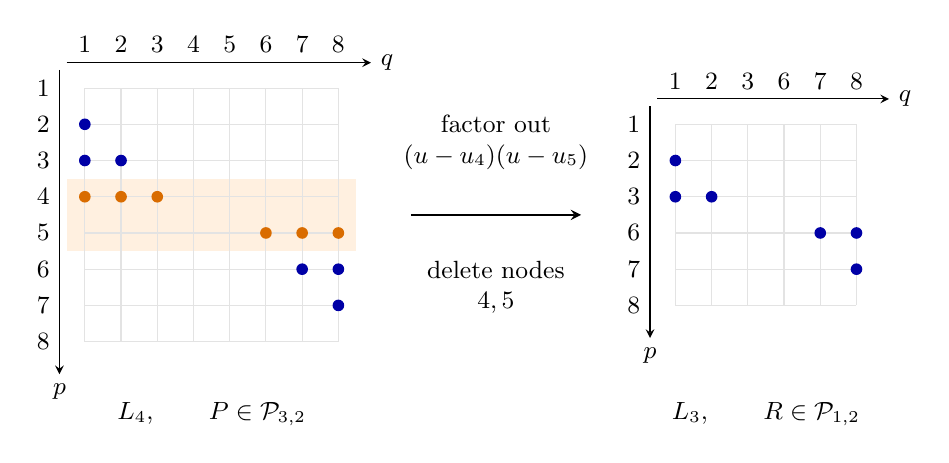
\begin{tikzpicture}[x=.46cm,y=.46cm,>=stealth,font=\small,
  kept/.style={fill=blue!65!black},
  removed/.style={fill=orange!85!black}]
  \begin{scope}
    \fill[orange!12] (.5,-5.5) rectangle (8.5,-3.5);
    \draw[step=1,gray!22] (1,-8) grid (8,-1);
    \draw[->] (.5,-.3)--(8.9,-.3) node[right] {$q$};
    \draw[->] (.3,-.5)--(.3,-8.9) node[below] {$p$};
    \foreach \i in {1,...,8} {
      \node[above] at (\i,-.3) {$\i$};
      \node[left] at (.3,-\i) {$\i$};
    }
    \foreach \p/\q in {2/1,3/1,3/2,6/7,6/8,7/8}
      \fill[kept] (\q,-\p) circle (2.1pt);
    \foreach \p/\q in {4/1,4/2,4/3,5/6,5/7,5/8}
      \fill[removed] (\q,-\p) circle (2.1pt);
    \node at (4.5,-10) {$L_4,\qquad P\in\mathcal P_{3,2}$};
  \end{scope}
  \draw[->,line width=.65pt] (10,-4.5)--(14.7,-4.5);
  \node[align=center] at (12.35,-2.5)
    {factor out\\$(u-u_4)(u-u_5)$};
  \node[align=center] at (12.35,-6.5)
    {delete nodes\\$4,5$};
  \begin{scope}[xshift=7.5cm,yshift=-.46cm]
    \draw[step=1,gray!22] (1,-6) grid (6,-1);
    \draw[->] (.5,-.3)--(6.9,-.3) node[right] {$q$};
    \draw[->] (.3,-.5)--(.3,-6.9) node[below] {$p$};
    \foreach \i/\j in {1/1,2/2,3/3,4/6,5/7,6/8} {
      \node[above] at (\i,-.3) {$\j$};
      \node[left] at (.3,-\i) {$\j$};
    }
    \foreach \p/\q in {2/1,3/1,3/2,4/5,4/6,5/6}
      \fill[kept] (\q,-\p) circle (2.1pt);
    \node at (3.5,-9) {$L_3,\qquad R\in\mathcal P_{1,2}$};
  \end{scope}
\end{tikzpicture}
\caption{The two-triangle interpolation pattern for eight nodes.
The axes record indices, not the numerical sizes of the nodes. Each
highlighted row has three points, so a polynomial
$P\in\mathcal P_{3,2}$ vanishing on $L_4$ vanishes identically on both
rows. Dividing by $(u-u_4)(u-u_5)$ gives
$R\in\mathcal P_{1,2}$, the swapped degree rectangle for six nodes.
After deleting indices $4,5$, the remaining points form $L_3$;
the right panel retains their original labels.}
\label{fig:interpolation}
\end{figure}


Fix any linear order of the \(2s\) nodes, and write
\[
S(p,q)=
\begin{cases}
\tfrac12,&p\text{ precedes }q,\\
-\tfrac12,&q\text{ precedes }p,\\
0,&p=q.
\end{cases}
\]
Using the polynomial \(G\) from Lemma~\ref{lem:weights}, define
\begin{equation}\label{eq:M}
M(A,B)=\sum_{p,q}
S(p,q)\frac{u_p-u_q}{G'(u_p)G'(u_q)}
A(u_p,u_q)B(u_p,u_q).
\end{equation}

\begin{lemma}[Order detection]\label{lem:detector}
The pairing \(M\) on
\(\PP_{s-1,s-2}\times\PP_{s-2,s-1}\) is nonsingular.
Consequently,
\begin{equation}\label{eq:detector}
A\in\PP_{s-2,s-2},\quad
M(A,B)=0\ \text{for every }B\in\PP_{s-1,s-1}
\quad\Longrightarrow\quad A=0.
\end{equation}
\end{lemma}

\begin{proof}
Let \(A\in\PP_{s-1,s-2}\) and \(B\in\PP_{s-2,s-1}\).
The product \((u-v)A(u,v)B(u,v)\) has degree at most \(2s-2\)
in each variable. Consequently, replacing \(S(p,q)\) by
\(S(p,q)+r_p+c_q\) leaves \(M(A,B)\) unchanged: the added
\(r_p\) terms vanish after the weighted sum in \(q\), by
Lemma~\ref{lem:weights}, and the \(c_q\) terms vanish after
the weighted sum in \(p\). Diagonal entries have no effect
because \(u_p-u_q=0\) there.

Relabel the nodes in their prescribed order; their numerical values
remain arbitrary distinct real numbers. Off the diagonal,
\(S(p,q)=\tfrac12-\mathbf1_{\{q<p\}}\). We may therefore replace
\(S\) in the pairing by
\[
K(p,q)=
\begin{cases}
-1,&1\le q<p\le s,\\
 1,&s<p<q\le2s,\\
 0,&\text{otherwise}.
\end{cases}
\]
Indeed, off the diagonal this is
\(S(p,q)-\tfrac12+\mathbf1_{\{p>s\}}\), an allowed change by
a row term and a constant. Hence
\[
M(A,B)=\sum_{(p,q)\in L_s}
K(p,q)\frac{u_p-u_q}{G'(u_p)G'(u_q)}
A(u_p,u_q)B(u_p,u_q).
\]
Every displayed weight is nonzero. Lemma~\ref{lem:triangles}
identifies each of the two polynomial spaces with \(\R^{L_s}\)
by evaluation. In these two coordinate systems the pairing is
diagonal with nonzero entries, so it is nonsingular.

For the consequence, the smaller space for \(A\) is contained
in the first nonsingular space, while the given test space for
\(B\) contains the second one. Nonsingularity forces \(A=0\).
\end{proof}

\section{The lower bound}\label{sec:lower}

Assume first that \(n=2s+1\ge5\). Fix a normalized minimum drawing,
label its vertices \(1,\ldots,n\), and form \(J\) as in
Equation~\eqref{eq:J}. Choose distinct real labels \(t_1,\ldots,t_n\)
and set
\[
F(t)=\prod_{i=1}^{n}(t-t_i),\qquad w_i=\frac1{F'(t_i)}.
\]

\begin{lemma}[Polynomial cycle tests]\label{lem:tests}
For every polynomial \(H(x,u,y,v)\) of degree at most \(n-2\)
separately in each variable,
\begin{equation}\label{eq:test}
\sum_{i,p,k,q}
J([ip],[kq])w_iw_pw_kw_q H(t_i,t_p,t_k,t_q)=0.
\end{equation}
\end{lemma}

\begin{proof}
For exponents \(a,b\le n-2\), the chain
\[
z_{a,b}=\sum_{i,p}w_iw_p t_i^a t_p^b[ip]
\]
has boundary
\[
\left(\sum_iw_i t_i^a\right)\sum_pw_p t_p^b\ee_p
-
\left(\sum_pw_p t_p^b\right)\sum_iw_i t_i^a\ee_i=0
\]
by Lemma~\ref{lem:weights}. For a monomial
\(H=x^au^by^cv^h\), Equation~\eqref{eq:test} is
\(J(z_{a,b},z_{c,h})=0\), by Lemma~\ref{lem:cycles}.
Linearity gives the result.
\end{proof}

Let \(\TT\) be the set of \emph{ordered pairs of undirected edges}
that have no common endpoint and have nonzero signed crossing
count \(J\). This condition does not depend on the chosen edge
orientations. Each coordinate records an edge pair, which may cross
repeatedly.
Each unordered supported pair requires at least
one crossing, so
\begin{equation}\label{eq:support}
c(D)\ge\frac{|\TT|}{2}.
\end{equation}

Let \(\SSS\) be the space of polynomials \(P(x,u,y,v)\) with
degree at most \(s-2\) separately in each variable, symmetric
within \((x,u)\) and within \((y,v)\). Symmetry under exchanging
the two pairs is \emph{not} imposed. A symmetric polynomial
in one pair has a basis indexed by exponent pairs
\(0\le a\le b\le s-2\). Hence
\begin{equation}\label{eq:dim}
\dim\SSS=\binom{s}{2}^{\!2}.
\end{equation}
The evaluation map
\[
E:\SSS\longrightarrow\R^\TT,\qquad
E(P)_{(\{i,p\},\{k,q\})}=P(t_i,t_p,t_k,t_q)
\]
is well-defined by the two within-pair symmetries. We will first prove
that these evaluations determine every polynomial in \(\SSS\). We will
then use the cycle identity a second time to show that their image
has dimension at most half the number of coordinates.

\begin{lemma}[Injectivity]\label{lem:injectivity}
The map \(E\) is injective.
\end{lemma}

\begin{proof}
Suppose \(E(P)=0\). We first force vanishing at a shared endpoint,
then use the resulting polynomial factors to descend in degree.

\emph{Localizing at a shared endpoint.} In Lemma~\ref{lem:tests} use
\begin{equation}\label{eq:localtest}
H=P(x,u,y,v)(u-v)(u-y)(v-x)U(x)V(y)B(u,v),
\end{equation}
where \(\deg U,\deg V\le s\) and \(B\in\PP_{s-1,s-1}\).
The three-factor weight has separate degrees \((1,2,1,2)\);
the total degrees are therefore at most \(2s-1=n-2\).

Independent-edge terms vanish either by \(E(P)=0\) or by their
zero \(J\). The weight kills the coincidences \(p=q\), \(p=k\),
and \(q=i\); loops already have zero edge vector. Only \(i=k\)
survives, with \(p,q\) distinct from \(i\) and from each other.
Since adjacent edges do not cross and both orientations point out
of \(i\),
\[
J([ip],[iq])=\tfrac12 T_i(ip,iq)=:S_i(p,q).
\]
Set \(S_i(p,p)=0\) and \(F_i(t)=\prod_{p\ne i}(t-t_p)\).
For \(p\ne i\),
\((t_p-t_i)w_p=1/F_i'(t_p)\), so Equation~\eqref{eq:test} becomes
\begin{equation}\label{eq:local}
0=\sum_i w_i^2U(t_i)V(t_i)
\sum_{\substack{p\ne i\\q\ne i}}
S_i(p,q)\frac{t_p-t_q}{F_i'(t_p)F_i'(t_q)}
P(t_i,t_p,t_i,t_q)B(t_p,t_q).
\end{equation}

For each fixed \(B\), products \(U(t)V(t)\) span all polynomials
of degree at most \(2s=n-1\): split each monomial's exponent
into two parts of size at most \(s\). Their linear combinations
interpolate arbitrary values on the \(n\) nodes. Since \(w_i\ne0\),
the inner sum in Equation~\eqref{eq:local} vanishes separately
for every \(i\) and every \(B\). More explicitly, for fixed \(B\),
linearity allows \(U V\) to be replaced by the Lagrange polynomial
that is one at \(t_i\) and zero at all other nodes. For each \(i\),
the inner sum is the order pairing on the \(2s\) nodes different
from \(t_i\). Its first polynomial,
\(P(t_i,u,t_i,v)\), belongs to \(\PP_{s-2,s-2}\).
Lemma~\ref{lem:detector} gives
\[
P(t_i,u,t_i,v)=0
\quad\text{as a polynomial in }u,v,\quad\text{for every }i.
\]

\emph{Dividing the collision factors.} The polynomial \(P(x,u,x,v)\)
has degree at most \(2s-4<n\) in \(x\).
Applying the univariate root bound to each coefficient in \(u,v\)
shows that it is identically zero. Hence \(x-y\) divides \(P\).
The two within-pair symmetries imply divisibility also by
\(x-v\), \(u-y\), and \(u-v\). Each difference is prime: quotienting
the polynomial ring by that factor identifies its two variables
and leaves a polynomial ring,
which has no zero divisors. The four factors are pairwise nonassociate,
so their individual divisibility implies divisibility by their product
\begin{equation}\label{eq:C}
C=(x-y)(x-v)(u-y)(u-v).
\end{equation}

We have proved that \(C\) divides every polynomial in the kernel.
For a nonzero polynomial, this already forces every separate degree
to be at least two. If the kernel contains a nonzero polynomial,
choose \(P\) of minimum degree in \(x\) and write \(P=CR\)
with \(R\ne0\).
The product \(C\) is invariant under each within-pair swap;
applying either swap and cancelling \(C\) shows that \(R\)
has the same two symmetries. Its degree in each variable is two
less than that of \(P\), so \(R\in\SSS\).
Moreover, \(C\) is nonzero at every evaluated independent-edge pair,
so \(E(R)=0\). This contradicts the minimal choice of \(P\).
\end{proof}

\begin{proposition}[Odd lower bound]\label{prop:odd}
Every normalized minimum drawing of \(K_{2s+1}\), \(s\ge2\),
has at least \(\binom{s}{2}^{2}\) crossings.
\end{proposition}

\begin{proof}
Define the full difference product
\[
\Delta=(x-u)(y-v)(x-y)(x-v)(u-y)(u-v).
\]
For \(P,Q\in\SSS\), the polynomial \(PQ\Delta\) has separate degrees
at most \(2(s-2)+3=2s-1\), so Lemma~\ref{lem:tests} applies.
Its only nonzero terms come from \(\TT\): every common endpoint
kills \(\Delta\).

Fix representative orientations for the edges. For each ordered
pair in \(\TT\), its four choices of endpoint orientations give
equal contributions. Reversing either edge changes the signs of
both \(J\) and \(\Delta\), while leaving \(P,Q\) and the node-weight
product unchanged. After division by four,
\[
\sum_{\alpha\in\TT}a_\alpha E(P)_\alpha E(Q)_\alpha=0,
\quad
a_{(\{i,p\},\{k,q\})}
=J([ip],[kq])w_iw_pw_kw_q
\Delta(t_i,t_p,t_k,t_q).
\]
Every \(a_\alpha\) is nonzero, so this is a nondegenerate
\emph{symmetric diagonal} form on \(\R^\TT\).
In particular it is not the skew form \(J\). Exchanging the two
whole edges gives a different coordinate with opposite coefficient,
a block \(\operatorname{diag}(a,-a)\); this does not destroy
nondegeneracy.

The image \(W=E(\SSS)\) is contained in its orthogonal complement.
To justify the dimension count, let \(V=\R^\TT\). The nondegenerate
form identifies \(V\) with its dual. Restricting a linear functional
on \(V\) to \(W\) is onto \(W^*\), since any basis of \(W\) extends
to a basis of \(V\). The resulting map \(V\to W^*\) has kernel
\(W^\perp\); hence
\(\dim W^\perp=|\TT|-\dim W\), and therefore
\(2\dim W\le|\TT|\).
By Lemma~\ref{lem:injectivity} and Equations~\eqref{eq:support}
and~\eqref{eq:dim},
\[
c(D)\ge\frac{|\TT|}{2}\ge\dim W=\binom{s}{2}^{\!2}.
\]
Cancellation of signs at repeated crossings can only remove
coordinates from \(\TT\), and so cannot invalidate this inequality.
\end{proof}

\begin{corollary}\label{cor:lower}
For every \(n\ge3\), \(\crn(K_n)\ge Z(n)\).
\end{corollary}

\begin{proof}
Proposition~\ref{prop:odd} proves the odd cases \(n\ge5\).
For \(n=2s>4\), delete each vertex in turn from a normalized
minimum drawing. Every crossing involves four distinct vertices,
so survives exactly \(n-4\) deletions. Each remaining drawing of
\(K_{n-1}\), whether minimum or not, has at least
\(\binom{s-1}{2}^{2}\) crossings. Thus
\[
(n-4)c(D)\ge n\binom{s-1}{2}^{\!2},
\qquad
c(D)\ge\frac{s(s-1)^2(s-2)}4.
\]
For \(n=3,4\), nonnegativity gives the claimed zero lower bound.
\end{proof}

\section{A matching two-page drawing}\label{sec:upper}

We use the endpoint-sum construction presented by de Klerk, Pasechnik,
and Salazar~\cite[Section~5.1]{DPSBookPreprint}, which builds on the
book drawings of Bla\v{z}ek and Koman~\cite{BlazekKoman1964} and of
Damiani, D'Antona, and Salemi~\cite{DamianiEtAl1994}.
Its two-page case attains the classical upper bound.
The vertices lie on a line, called the \emph{spine}, and each edge lies
in one of its two half-planes. We count the crossings directly,
including the parity issue in the cyclic enumeration.

Place the vertices with labels \(0,\ldots,n-1\) at positions
\((a_0,0),\ldots,(a_{n-1},0)\), where
\(a_0<\cdots<a_{n-1}\). Put \(m=\lfloor n/2\rfloor\).
Color the residues \(0,\ldots,m-1\) with one color and
\(m,\ldots,n-1\) with another. An edge \(ij\) uses the color of
\(i+j\pmod n\). Draw first-color edges as semicircles above the
spine and second-color edges as semicircles below it, in both cases
with their endpoints as the diameter endpoints.

Two edges in different half-planes have disjoint interiors. In one
half-plane, two semicircles cross exactly when their four endpoints
alternate along the spine, and then they cross once. Indeed, the
semicircle with endpoints \(a<b\) satisfies
\[
 y^2=(x-a)(b-x).
\]
The difference of the two right-hand sides is affine in \(x\).
For four distinct endpoints, at the ends of the overlap of the
diameter intervals its signs are opposite for alternating endpoints and agree for nested intervals;
disjoint intervals have no overlap. This also shows that arcs
sharing an endpoint meet only there. Every interior
intersection is transverse: two circles with centers on the spine
can be tangent only at a point of the spine.

Choose the positions generically to exclude triple interior
crossings. For completeness, choose each \(a_i\) successively in a
prescribed open interval, with these intervals pairwise disjoint
and ordered from left to right. A triple interior crossing would
involve six distinct endpoints, since edges sharing an endpoint
have no other intersection. When the last of these endpoints is
placed, its partner \(a\) and a possible intersection \((x,y)\),
\(y\ne0\), of the other two semicircles are already fixed. If
\(x=a\), no such semicircle exists. Otherwise the unknown endpoint
\(b\) must satisfy
\[
 b=x+\frac{y^2}{x-a},
\]
which excludes at most one position for \(b\). There are only finitely many choices
to exclude. Thus the resulting drawing is admissible, and its
crossings are precisely the same-color pairs with alternating
endpoints. This alternation depends only on the cyclic order of the
labels \(0,\ldots,n-1\), which we use in the count below.

Figure~\ref{fig:two-page} shows the construction for \(n=7\).
\begin{figure}[tbp]
\centering
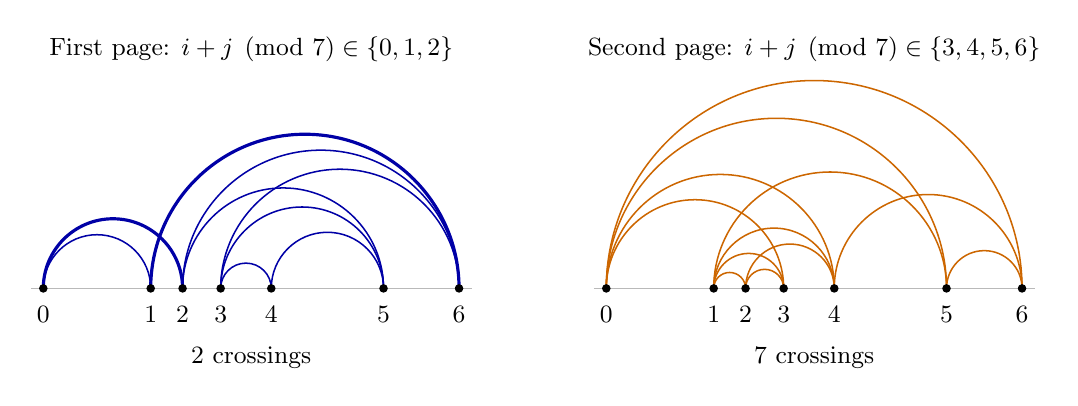
\begin{tikzpicture}[x=.88cm,y=.88cm,font=\small,
  spine/.style={draw=gray!55,line width=.35pt},
  first/.style={draw=blue!65!black,line width=.55pt},
  second/.style={draw=orange!80!black,line width=.55pt}]
  \def\positions{0/0,1/1.55,2/2.01,3/2.56,4/3.29,5/4.91,6/6}
  \begin{scope}
    \node[align=center] at (3,3.45)
      {First page: $i+j\pmod 7\in\{0,1,2\}$};
    \draw[spine] (-.18,0)--(6.18,0);
    \foreach \a/\b in {0/1.55,2.01/4.91,2.01/6,2.56/3.29,2.56/4.91,2.56/6,3.29/4.91} {
      \pgfmathsetmacro{\rad}{(\b-\a)/2}
      \draw[first] (\a,0) arc[start angle=180,end angle=0,radius=\rad];
    }
    \foreach \a/\b in {0/2.01,1.55/6} {
      \pgfmathsetmacro{\rad}{(\b-\a)/2}
      \draw[first,line width=1.15pt] (\a,0) arc[start angle=180,end angle=0,radius=\rad];
    }
    \foreach \i/\x in \positions {
      \fill (\x,0) circle (1.55pt);
      \node[below=3pt] at (\x,0) {$\i$};
    }
    \node at (3,-1.0) {$2$ crossings};
  \end{scope}
  \begin{scope}[xshift=7.15cm]
    \node[align=center] at (3,3.45)
      {Second page: $i+j\pmod 7\in\{3,4,5,6\}$};
    \draw[spine] (-.18,0)--(6.18,0);
    \foreach \a/\b in {0/2.56,0/3.29,0/4.91,0/6,1.55/2.01,1.55/2.56,1.55/3.29,1.55/4.91,2.01/2.56,2.01/3.29,3.29/6,4.91/6} {
      \pgfmathsetmacro{\rad}{(\b-\a)/2}
      \draw[second] (\a,0) arc[start angle=180,end angle=0,radius=\rad];
    }
    \foreach \i/\x in \positions {
      \fill (\x,0) circle (1.55pt);
      \node[below=3pt] at (\x,0) {$\i$};
    }
    \node at (3,-1.0) {$7$ crossings};
  \end{scope}
\end{tikzpicture}
\caption{The two-page construction for $K_7$. The pages are displayed
separately on the same labeled spine; reflect the second panel below
the spine to assemble the drawing. Page membership is determined by
the endpoint sum modulo $7$. The highlighted first-page edges $02$ and
$16$ cross because $0<1<2<6$. The displayed semicircles have $2$ and
$7$ distinct crossings.}
\label{fig:two-page}
\end{figure}


\begin{proposition}\label{prop:upper}
This drawing has exactly \(Z(n)\) crossings for every \(n\ge3\).
\end{proposition}

\begin{proof}
Each four-set of vertices has one alternating edge pair, its
diagonals. Count cyclic tuples starting at a label \(a\), with
successive positive integer gaps \(g_1,g_2,g_3,g_4\) summing to \(n\).
The four vertices are
\[
 a,\quad a+g_1,\quad a+g_1+g_2,\quad a+g_1+g_2+g_3
 \pmod n.
\]
Each four-set occurs four times, once for each starting vertex.
The diagonal endpoint-sum residues are
\[
r=2a+g_1+g_2,\qquad r+k,\qquad k=g_1+g_3.
\]
For \(2\le k\le n-2\), put \(\ell=\min(k,n-k)\), and let \(R_k\)
be the residues \(r\) for which \(r,r+k\) have the same color.
Shifting by \(\ell\le m\) changes color on \(\ell\) residues from
each block, so
\[
|R_k|=n-2\ell.
\]
For each \(k\) there are \((k-1)(n-k-1)\) gap choices:
choose \(1\le g_1\le k-1\) and \(1\le g_2\le n-k-1\);
the other gaps are determined.

We claim that, including all \(a\), the number of same-color
tuples for this \(k\) is
\begin{equation}\label{eq:gapcount}
(k-1)(n-k-1)|R_k|.
\end{equation}
For odd \(n\), multiplication by two permutes the residues, so
each fixed gap choice already contributes \(|R_k|\).
For even \(n=2m\), as \(a\) varies, \(r=2a+g_1+g_2\) visits each
residue in the parity class of \(g_1+g_2\) twice. We must check that this restriction still gives
Equation~\eqref{eq:gapcount} after summing over the gap choices.
There are three cases.
If \(m\) is odd, \(R_k\) is invariant under adding \(m\), which
switches parity, so its parity classes have equal sizes.
If \(m,k\) are both even, \(R_k\) consists of two cyclic intervals
of even length \(m-\ell\), and again has equal parity counts.
Finally, if \(m\) is even and \(k\) odd, the \(k-1\) choices for
\(g_1\), for each fixed \(g_2\), give both parities of \(g_1+g_2\)
equally often. Averaging their doubled parity-class counts proves
Equation~\eqref{eq:gapcount} in this case too.

Dividing the total by four, and pairing \(k\) with \(n-k\), gives
\begin{align*}
c(D)
&=\frac14\sum_{k=2}^{n-2}
(k-1)(n-k-1)\bigl(n-2\min(k,n-k)\bigr)\\
&=\frac12\sum_{k=1}^{m}
(k-1)(n-k-1)(n-2k).
\end{align*}
The added \(k=1\) term is zero, as is the possible central
term \(k=n/2\). Set
\[
B_k=k(k-1)(n-k-1)(n-k-2).
\]
A direct subtraction gives
\[
B_k-B_{k-1}=2(k-1)(n-k-1)(n-2k).
\]
Since \(B_0=0\), the crossing count is \(c(D)=B_m/4\).
For \(n=2m+1\) this is \(m^2(m-1)^2/4\); for \(n=2m\)
it is \(m(m-1)^2(m-2)/4\). These are \(Z(n)\), including
the zero values at \(n=3,4\).
\end{proof}

Corollary~\ref{cor:lower} and Proposition~\ref{prop:upper}
complete the proof of Theorem~\ref{thm:main}.

\appendix
\section{Normalization of continuous-arc drawings}\label{sec:normalization}

The following reduction, also used in \cite[Appendix~A]{BipartiteCompanion},
ensures that the lower bound applies to ordinary crossing number.
Removing adjacent-edge crossings is a standard reduction in this
setting~\cite{FulekEtAl2012}; the proof below includes the details
for continuous arcs.

\begin{lemma}\label{lem:normalization}
For every finite simple graph, a minimum ordinary drawing can be
chosen polygonal, straight near every vertex and crossing, and
without crossings between edges having a common endpoint.
\end{lemma}

\begin{proof}
Drawings with finitely many crossings exist, so their crossing
counts have a least nonnegative integer value, attained by a
drawing. Start with such a minimum drawing, and call its vertices
and crossings \emph{marks}. Parameterize every edge injectively
on \([0,1]\). On each edge choose pairwise disjoint relative
parameter neighborhoods, with disjoint closures, of its marked
parameters, one-sided at its endpoints.

Choose pairwise disjoint small closed round disks centered at the
marks. They can be made so small that every visit of an edge to
a disk lies in the corresponding parameter neighborhood, and
nonincident edges avoid it. Indeed, the image of the compact
parameter set outside that neighborhood avoids the mark, so has
positive distance from it; if the mark is not on the edge, use
the entire compact edge. There are finitely many such conditions.

For an interior mark, remove the edge passage from its first to
its last visit to the closed disk, including all intermediate
excursions. At an initial vertex remove through the last visit;
at a terminal vertex remove from the first visit. These intervals
are disjoint along each edge. The retained middle pieces are
finitely many pairwise disjoint compact arcs with distinct
boundary endpoints and interiors outside all closed disks.
This step does not require finitely many visits to a circle.

Choose pairwise disjoint open neighborhoods of the middle pieces.
At a boundary endpoint take a short radial spur out of its disk.
The spur tip can be joined to a nearby interior point of the
original middle piece within the chosen neighborhood and the open
exterior of all disks: a sufficiently small exterior collar sector
at that endpoint contains both points, and radial paths with a
short concentric arc join them. Do this at both ends and use the
middle piece between the selected interior points.

A compact path in an open subset of the plane has a polygonal
replacement there with the same endpoints: cover its image by
small balls inside the open set, subdivide its parameter interval
so that each subarc lies in one ball, and use chords in those balls.
Apply this between the spur tips and append the spurs.
Subdivide the finite union of segments at intersections and
endpoints, also splitting and identifying collinear overlaps.
A simple path in the resulting finite embedded graph gives a
simple polygonal replacement. The disjoint neighborhoods ensure
that the different exterior pieces do not meet.

In each crossing disk join its respective endpoint pairs by
straight chords. Their four boundary endpoints are distinct, so
the chords have at most one crossing, transverse if present.
In each vertex disk use straight spokes to its center; distinct
boundary endpoints give distinct rays, so the spokes meet only
at the vertex. Reassembling in the original edge order gives
simple edges: an edge uses at most one strand in each disk,
and all exterior pieces are disjoint. Every crossing lies in
an old crossing disk, with at most one there. The result is
polygonal and has no greater crossing count; hence it is minimum.

Suppose two edges \(vu,vw\) cross. Around one such crossing take
a small disk containing only their straight crossing strands.
Exchange the prefixes from \(v\) up to that disk and join them
to the original suffixes by disjoint chords. The new pairing
is nonalternating. We obtain two walks with the required endpoints
and with that crossing removed; outside the disk the two old
tracks are used exactly once in total.

Subdivide at bends and remaining intersections, and erase closed
subwalks between repeated subdivision vertices until both walks
are simple. At an old crossing of these two edges, either its
two tracks belong to different new walks, in which case each
retained passage remains straight, or both belong to one walk.
Only in the latter case can loop erasure make a turn, and neither
the other walk nor a third edge is present at that point.
A crossing with a third edge lies on a track visited at most
once by the two walks together, so any retained passage there
also remains straight. No new intersection, overlap, or improper
contact is introduced; all interiors still avoid graph vertices.
This gives an admissible drawing with fewer crossings, a
contradiction. Thus the polygonal minimum has no adjacent-edge
crossings.
\end{proof}

\begingroup
\raggedright
\bibliographystyle{plain}
\bibliography{references}
\endgroup
\end{document}
